% Slide 213
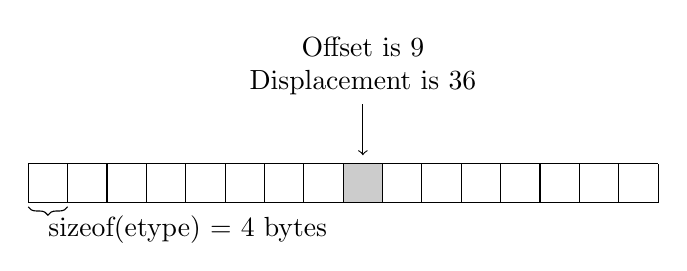
\begin{tikzpicture}
\draw[step = 0.5cm] (0,0) grid (8, 0.5);

\node[rectangle, draw, inner sep = 0.25cm, fill = gray!40!white, outer sep = 3pt] (R) at (4.25, 0.25) {};
\node[align = center, anchor = south] (W) at (4.25, 1.25) {Offset is 9 \\ Displacement is 36};

\draw[<-] (R) -- (W);

\draw[decorate,decoration={brace,amplitude=3pt, mirror}] (0, -0.05) -- (0.5, -0.05);
\node[anchor = north west, inner sep = 0pt] at (0.25, -0.15) {sizeof(etype) = 4 bytes};

\end{tikzpicture}
